\documentclass[12pt]{article}
\usepackage{bm}
\usepackage{graphicx}
\usepackage{gensymb}
\usepackage{float}
\usepackage{siunitx}
\usepackage[a4paper, total={6in, 8in}]{geometry}

\graphicspath{{./../images/}}

\begin{titlepage}

\title{\textbf{Optimum Loft Angle for Greatest Carry Distance}}
\author{\textbf{Group D}\\
		Alison McIntosh\\
		Emily Dark\\
		Henry Archer\\
		Kyle Stewart\\
		Stuart Ballantyne}
\date{}

\end{titlepage}

\begin{document}

\begin{titlepage}
\maketitle
\thispagestyle{empty}
\pagebreak
\end{titlepage}

\pagenumbering{arabic}

\section{Abstract}
...


\section{Response}
...

\section{Theory and model}

\subsection{Assumptions}
The following assumptions are made throughout the report and model:
\begin{description}
  \item[$\cdot$] golf course is level and has no effect on trajectory;
  \item[$\cdot$] height of the tee is negligible;
  \item[$\cdot$] gravitational field strength is constant (\SI{9.81}{\metre\per\second^{2}}) and does not flucuate with height;
  \item[$\cdot$] driver is roughly a flat plate and strikes the ball precisely at the center, with no draw or fade;
  \item[$\cdot$] the mass of the club head is significantly greater than that of the shaft, so we consider the shaft's influence to be neglible;
  \item[$\cdot$] the golf ball is a Titleist Pro V1, with a mass of \SI{45.93}{\gram}, diameter of \SI{42.67}{\milli\metre}.

\end{description}

\subsection{Impact}
...
\pagebreak
\subsection{Flight}
\subsubsection{Simple golf ball}
A simple golf ball experiencing only weight may be modelled by the following system of differential equations;
\begin{equation} \label{simpleaccelx}
a_x=\frac{\partial v_x}{\partial t}=0
\end{equation}
\begin{equation} \label{simpleaccely}
a_y=\frac{\partial v_y}{\partial t}=-g
\end{equation}
where $g$ is the gravitional field strength.

Assuming the initial velocity is $v_0$ and the launch angle is $\theta$, equations (\ref{simpleaccelx}-\ref{simpleaccely}) can be solved to give equations (\ref{simplevelx}-\ref{simplevely}):
\begin{equation} \label{simplevelx}
v_x=v_0 \cos{\theta}
\end{equation}
\begin{equation} \label{simplevely}
v_y=v_0 \sin{\theta}-gt
\end{equation}
Integrating equations (\ref{simplevelx}-\ref{simplevely}) with respect to time yields the displacement as a function of time:
\begin{equation} \label{simpleposx}
x=v_0 t \cos{\theta}
\end{equation}
\begin{equation} \label{simpleposy}
y=v_0 t \sin{\theta}-\frac{1}{2} g t^2
\end{equation}

\begin{figure}[H]
\centering
\caption{Golf ball trajectory, no drag or lift}
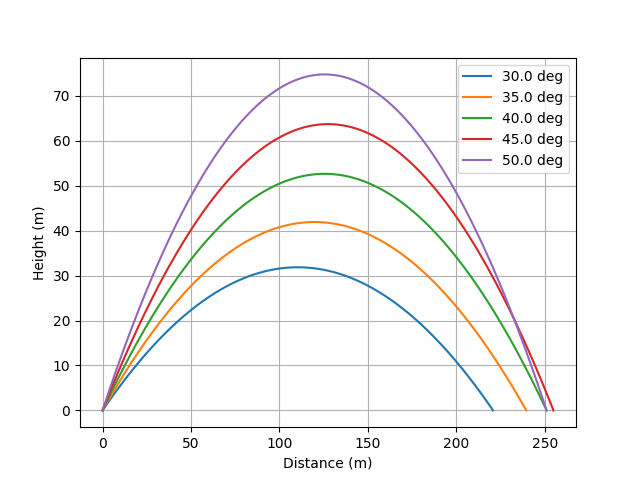
\includegraphics[scale=0.6]{simple}
\end{figure}

\begin{figure}[H]
\centering
\caption{Range as a function of loft angle, no drag or lift}
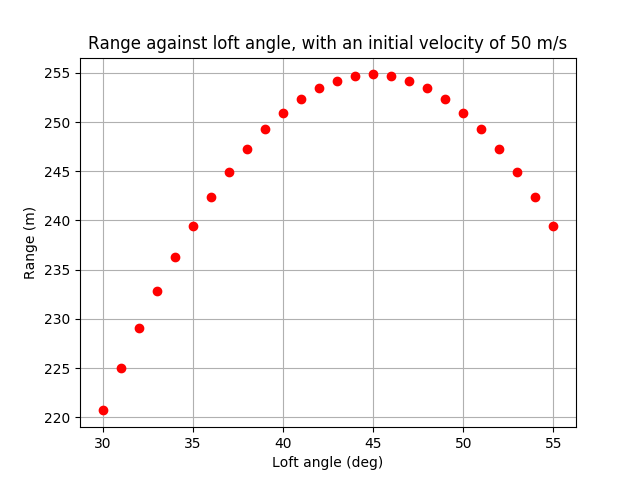
\includegraphics[scale=0.6]{simplerange}
\end{figure}

Figures (1-2) show the maximum range is when the loft angle at 45.0\degree, as predicted by the equations of projectile motion.

\subsubsection{Smooth golf ball experiencing drag}
The drag equation is given by:
\begin{equation} \label{drageqn}
\vec{F_{d}} = \frac{1}{2} A C_{d} \rho_{air} |\vec{v}| \vec{v}
\end{equation}
where $\rho_{air}$ is the density of air; $A$ is the reference area, which in the case of a smooth sphere of radius $r$, is the cross-sectional area $\pi r^2$; $C_d$ is the coefficient of drag, which is dependent on the Reynolds number; and $\vec{v}$ is the flow velocity relative to the golf ball. In this case, we assume the air is stationary and the golf ball is moving through the air with velocity $\vec{v}$.

Applying equation (\ref{drageqn}) to equations (\ref{simpleaccelx}-\ref{simpleaccely}), we get
\begin{equation} \label{dragaccelx}
\frac{\partial v_x}{\partial t}=-k |v_x| v_x
\end{equation}
\begin{equation} \label{dragaccely}
\frac{\partial v_y}{\partial t}=-g-k |v_y| v_y
\end{equation}
where $k=\frac{1}{2} A C_d \rho_{air}$.
\begin{figure}[H]
\centering
\caption{Golf ball trajectory when experiencing drag but no lift, $C_d=0.5$}
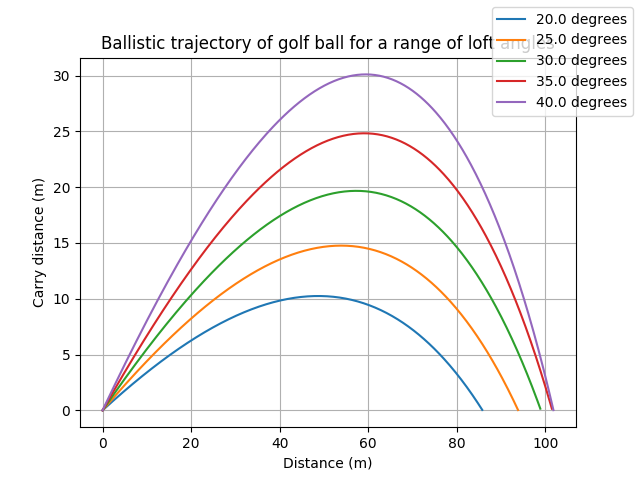
\includegraphics[scale=0.6]{dragcd}
\end{figure}

\begin{figure}[H]
\centering
\caption{Range as a function of loft angle, $C_d$ = 0.5}
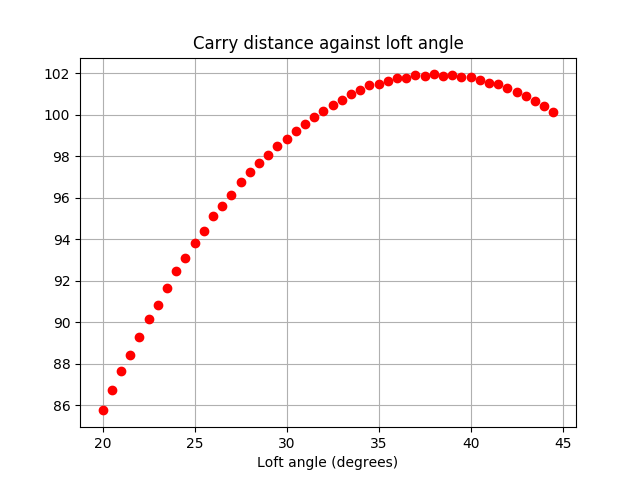
\includegraphics[scale=0.6]{dragcdrange}
\end{figure}

Figure (4) shows that the maximum range is achieved at 40.2\degree, for an initial velocity of \SI{50}{\metre\per\second}. Additionally, the range is significantly decreased when drag was added to the model. The greatest range with drag is about \SI{114}{\metre} versus the previous range of $255$ m at 45.0\degree.
However, $C_d$ is not constant and depends on the Reynolds number, which is proportional to the velocity of the golf ball. The Reynolds number is given by:
\begin{equation} \label{reynolds}
R=\frac{2vr}{\nu}
\end{equation}
where $\nu$ is the kinematic viscosity of air.

Using data from [whereever we found the Reynolds number data], we used Python to construct a quartic fit as shown in Figure (5). One of the limitions of this approach is that we did not have any data above Reynolds number $112,000$ (\SI{38.39}{\meter\per\second}) or below $63,300$ (\SI{21.70}{\meter\per\second}), so the approximation would not hold for those conditions, and may in fact be drastically worse due to the chaotic behaviour of the polynomial at those points. To get around this, the coefficient of drag is fixed at 0.8 for Reynolds numbers less than 53,000 and fixed at 0.37 for Reynolds numbers greater than 120,000.

\begin{figure}[H]
\centering
\caption{Coefficient of drag as a function of Reynolds number with curve of best fit}
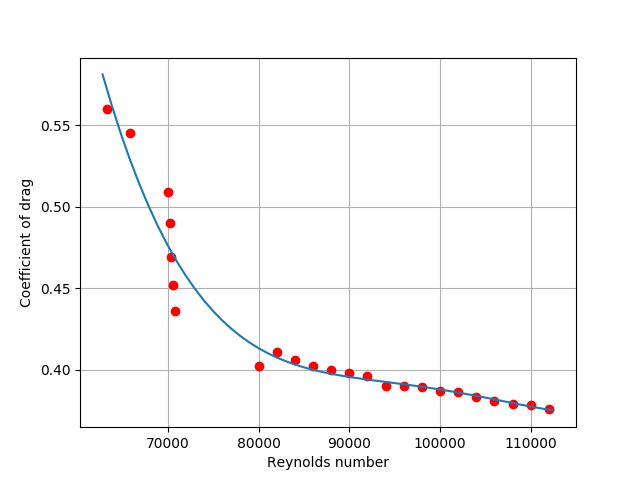
\includegraphics[scale=0.6]{reynolds}
\end{figure}

Applying the approxmation for the coefficient of drag, the optimum loft angle decreases down to about 34.5\degree, shown in figures (6-7).
\begin{figure}[H]
\centering
\caption{Trajectory of golf ball with drag considering Reynolds number, $v_i=50 m\cdot s^{-1}$}
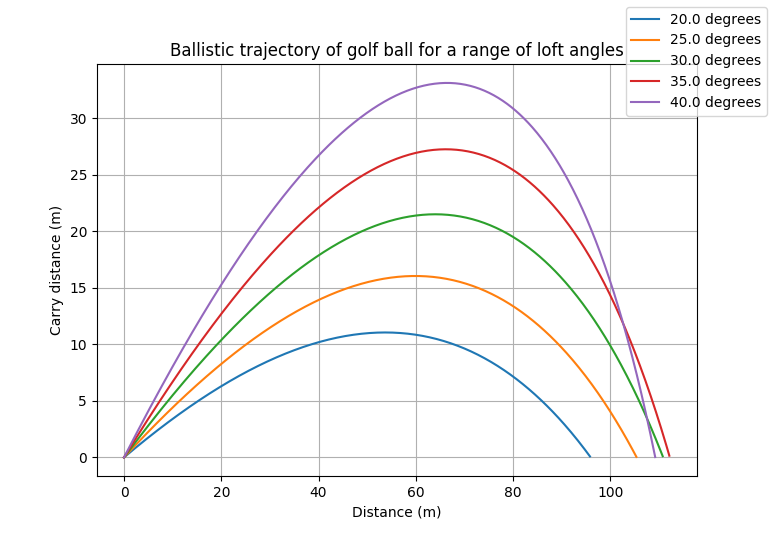
\includegraphics[scale=0.6]{dragwithreynolds}
\end{figure}

\begin{figure}[H]
\centering
\caption{Range against loft angle for golf ball with drag considering Reynolds number, $v_i=50 m\cdot s^{-1}$}
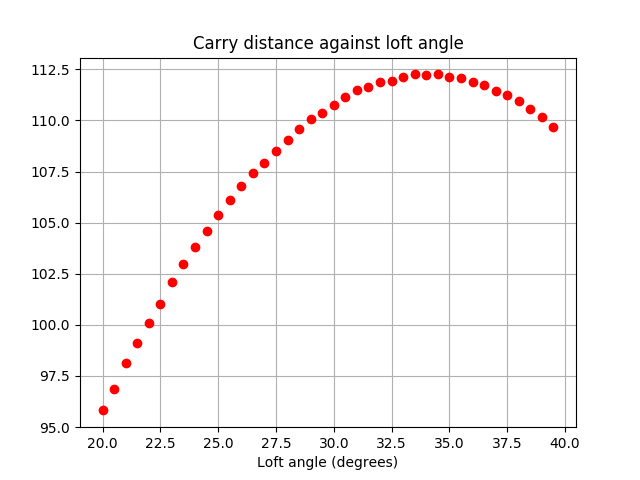
\includegraphics[scale=0.6]{dragwithreynoldsrange}
\end{figure}


\subsubsection{Smooth golf ball experiencing lift}
Lift on a golf ball is caused by the Magnus effect, which is dependent on the backspin of the ball. The equation is similar to the drag equation, however the direction of the force is perpendicular to both angular velocity and translational velocity, unlike in the drag equation.

\begin{equation} \label{lifteqn}
F_l = \frac{1}{2} \rho_{air} C_{l} |v|^2 (\hat{\omega} \times \hat{v})
\end{equation}

where $C_l$ is dependent on the spin parameter of the ball according to [whoever found this equation].
\begin{equation} \label{clifteqn}
C_l = -3.25 S^2 + 1.99 S
\end{equation}
The spin parameter is given by the ratio of the magnitude of tangential velocity to the magnitude of translational velocity.
\begin{equation} \label{spineqn}
S = \frac{r|\omega|}{|v|}
\end{equation}


\end{document}
\grid